\documentclass[a4paper]{article}

%% Language and font encodings
\usepackage[spanish]{babel}
\usepackage[utf8x]{inputenc}
\usepackage[T1]{fontenc}
\usepackage{listings}

%% Sets page size and margins
\usepackage[a4paper,top=3cm,bottom=2cm,left=3cm,right=3cm,marginparwidth=1.75cm]{geometry}

%% Useful packages
\usepackage{amsmath}
\usepackage{graphicx}
\usepackage[colorinlistoftodos]{todonotes}
\usepackage[colorlinks=true, allcolors=blue]{hyperref}

\title{Práctica 5: método Monte-Carlo}
\begin{document}
\maketitle

\section{Introducci\'on}
El objetivo de ésta prueba consiste en implementar el método Monte-Carlo en la aproximación del área bajo una curva, así mismo variar los parámetros de la prueba con el fin de observar si alguno de ellos ofrece una mayor precisión reflejada el resultado. Se comparó el resultado obtenido con el resultado que ofrece Wolfram Alpha (WA) con los mismos parámetros.

\section{Par\'ametros de Trabajo}
La experimentación se realizó en una iMac con procesador Intel(R)Core(TM) i5-6200U CPU 2.30 GHz 2.40 GHz con ocho GB en memoria RAM y sistema operativo Windows 10 Home.

Se establecieron los tamaños de muestra con un crecimiento exponencial, ya que cuando el aumento de puntos era de forma lineal la diferencia era muy poca y no se podía apreciar el efecto de los cambios. Para $n \in \{2^{10},2^{12},2^{14},2^{16},2^{18},2^{20},2^{22}\}$ con una reptición de veinte puntos, de lo cual cada punto representa el promedio de 200 aproximaciones, para los valores del intervalo de la integral fueron de $x \in [3,7]$ 

\begin{equation}
\int_{x=3}^{x=7} \dfrac{1}{e^x + e^{-x}} dx
\end{equation}

y el valor obtenido de la plataforma WA con el cual se comparó el error fue $0.00488341111$.
\section{Modificaciones del código}
Se creó una función para calcular el error o la diferencia entre los valores obtenidos con el registrado por WA, así mismo se crearon clusters con el fin de poder paralelizar lo más que se pudiera, utilizando siete de los núcleos de la máquina con el fin de que no perdiera su funcionalidad utilizandolos todos. Así mismo se midieron los tiempos de corrida para cada parámetro con la función $system.time$ y se crearon $data frames$ para guardar cada valor obtenido.

\begin{lstlisting}[frame=single]
error <-function(x){return(abs(x-known))}

cluster<-makeCluster(detectCores() - 1)
clusterExport(cluster,"generador")
clusterExport(cluster,"parte")
clusterExport(cluster,"desde")
clusterExport(cluster,"hasta")
\end{lstlisting}


\section{Resultados}
Se muestran a continuación figura 1,2 y 3 las cuales reflejan de un modo gráfico los comparativos y los resultados de la experimentación, para cada una de ellas se utilizó la escala que mejór reflejara los valores para todos los casos.


\begin{figure}[!]
\centering
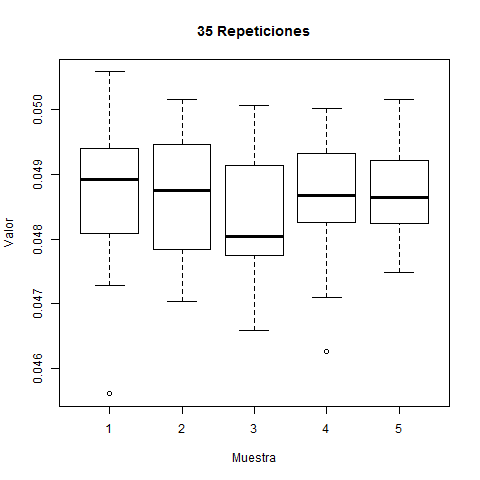
\includegraphics[width=0.7\linewidth]{aprox}
\caption{Aproximaciones al valor obtenido por WA, el cual es representado por la linea recta, para las diferentes cantidades de puntos}
\label{fig:aprox}
\end{figure}

\begin{figure}[!]
\centering
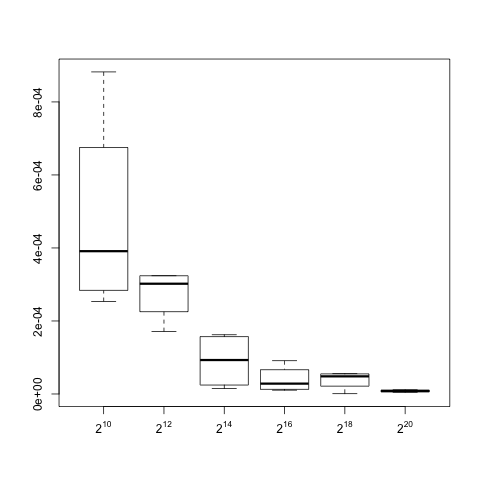
\includegraphics[width=0.7\linewidth]{error}
\caption{El error o diferencia obtenido para cada valor de puntos respecto al obtenido con WA}
\label{fig:error}
\end{figure}

\begin{figure}[!]
\centering
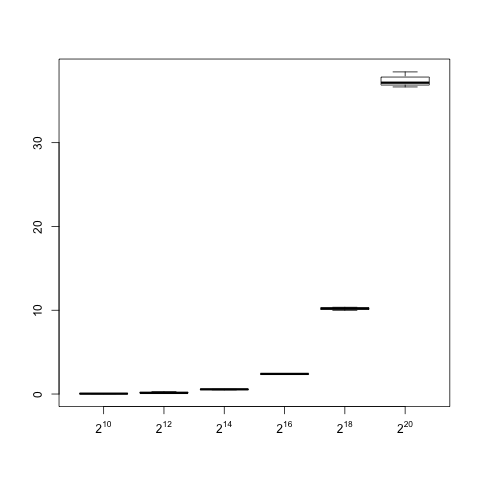
\includegraphics[width=0.7\linewidth]{tiempos}
\caption{El tiempo de computo para cada uno de los casos}
\label{fig:tiempos}
\end{figure}


\subsection{Interpretación}
En la figura 1 se observa que para los primeros valores de puntos, los cuales eran muy bajos y la aproximación del valor de el área era muy disperso, e incluso aunque sí se aproximaba al valor dado por WA la mayoría de los puntos no lo hacían, en cambio, al crecer la cantidad de puntos más allá del $2^{16}$ la disperción de los valores se reduce, así mismo la aproximación tiene una mayor presición.

En la figura 2 podemos reafirmar lo que se dijo de la figura 1, ya que en ésta figura representa el error que se tiene respecto al valor de WA, es decir, el valor absoluto de la diferencia de estas dos cifras. De igual modo se observa una notoria disminución del error a partir de $2^{16}$, puntualizando que ésta casi llega al cero en el valor de $2^{22}$ .

Comportamiento contrastante y como es de esperarse en la figura 3 podemos observar el modo de aumento en tiempos de ejecución para cada uno de los valores de puntos, el cual es medido en segundos. Hasta el valor de $2^{16}$ el tiempo de ejecución es relativamente pequeño, y podemos observar que no varía mucho de una replica a otra, pero al momento de llegar al valor de $2^{18}$ es cuando podemos observar el crecimiento de una manera más notoria.
 


\end{document}
